% This file was created by matlab2tikz.
%
%The latest updates can be retrieved from
%  http://www.mathworks.com/matlabcentral/fileexchange/22022-matlab2tikz-matlab2tikz
%where you can also make suggestions and rate matlab2tikz.
%
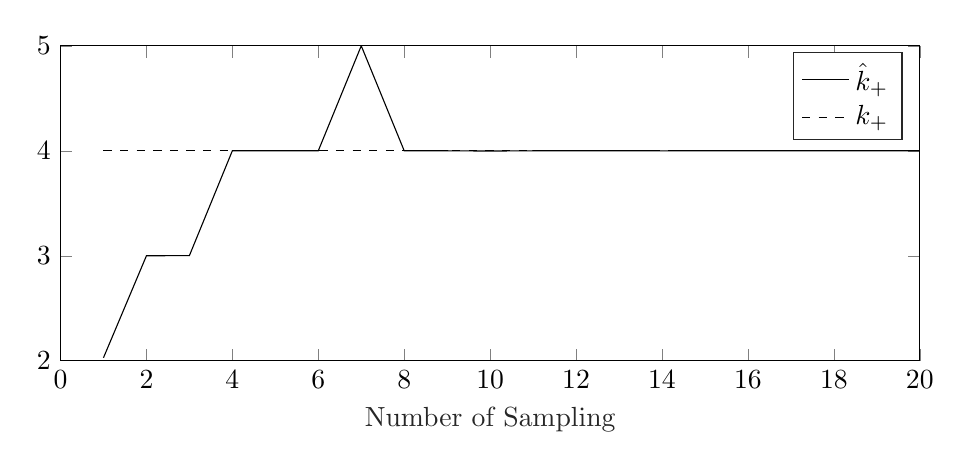
\begin{tikzpicture}

\begin{axis}[%
width=.9\linewidth,
height=4cm,
at={(0in,0in)},
scale only axis,
xmin=0,
xmax=20,
xlabel style={font=\color{white!15!black}},
xlabel={Number of Sampling},
ymin=2,
ymax=5,
ylabel style={font=\color{white!15!black}},
%ylabel={Number of Positive Eigenvalues},
axis background/.style={fill=white},
legend style={legend cell align=left, align=left, draw=white!15!black}
]
\addplot [color=black]
  table[row sep=crcr]{%
1	2.02878333228051\\
2	3.00000412526795\\
3	3.00194629230602\\
4	4.00051449032303\\
5	3.99998363733881\\
6	4.00013569715796\\
7	4.99994381698126\\
8	4.00000796483248\\
9	4.00001514241167\\
10	3.99769291363055\\
11	4.00000101918524\\
12	3.99998931573416\\
13	4.00031626976621\\
14	3.99993739195579\\
15	4.00000679714354\\
16	3.99999350520674\\
17	3.99999827766674\\
18	4.000001796798\\
19	4.00000216695133\\
20	4.00016721827853\\
};
\addlegendentry{$\hat{k}_+$}

\addplot [color=black, dashed]
  table[row sep=crcr]{%
1	4\\
20	4\\
};
\addlegendentry{$k_+$}

\end{axis}
\end{tikzpicture}%